\documentclass[12pt, twoside]{article}
\input{../preamble}

\fancyhead[LE]{\thepage}
\fancyhead[RO]{Markscheme}
\fancyhead[LO]{La Scuola d'Italia / Dr.\ Huson / IB Math 12 \\* 9 September 2026}

\begin{document}
\subsubsection*{2.1 Classwork: Exponential Functions Review ---
Markscheme}

\begin{enumerate}[itemsep=0.3cm]

%--- Problem 1: Exponential graph --- asymptote, intercepts, sketch [7 marks] ---
\item[1.] [Maximum mark: 7]

$f(x) = 3 \cdot 2^{\,x} - 5$.

\medskip

\textbf{(a)} As $x \to -\infty$, $2^{\,x} \to 0$, so $f(x) \to -5$.

Horizontal asymptote: $y = -5$. \hfill \textbf{A1}

\emph{Do not accept $-5$ alone: the answer is the equation of a line.}

\medskip

\textbf{(b)} $f(0) = 3 \cdot 2^{0} - 5 = 3 - 5 = -2$, so the
$y$-intercept is $(0, -2)$. \hfill \textbf{A1}

\emph{Accept $-2$.}

\medskip

\textbf{(c)} $f(4) = 3 \cdot 2^{4} - 5 = 48 - 5 = 43$.
\hfill \textbf{A1}

\medskip

\textbf{(d)} Set $f(x) = 0$: $\;3 \cdot 2^{\,x} = 5$, so
$2^{\,x} = \dfrac{5}{3}$. \hfill \textbf{M1}

$x = \log_{2}\!\left(\dfrac{5}{3}\right)
= \dfrac{\ln(5/3)}{\ln 2} = 0.736965\ldots$

$x \approx 0.737$ (3 s.f.) \hfill \textbf{A1}

\emph{Accept $(0.737,\, 0)$. Accept the exact form
$\log_{2}(5/3)$. A direct GDC solve of
$3 \cdot 2^{\,x} - 5 = 0$ earns the M1.}

\medskip

\textbf{(e)} Sketch: \hfill \textbf{A1A1}

\begin{center}
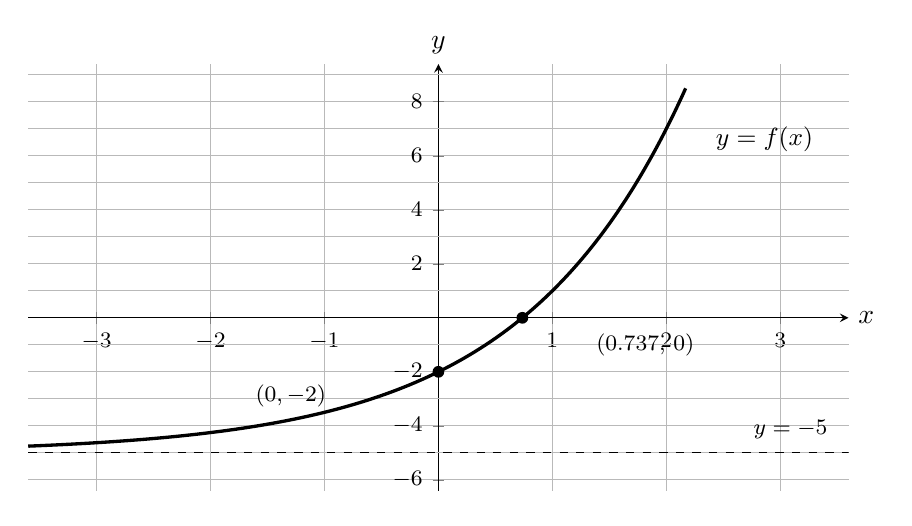
\begin{tikzpicture}
\begin{axis}[
  axis lines=middle,
  xlabel={$x$}, ylabel={$y$},
  xlabel style={anchor=west}, ylabel style={anchor=south},
  xmin=-3.6, xmax=3.6, ymin=-6.4, ymax=9.4,
  xtick={-3,-2,-1,1,2,3},
  ytick={-6,-4,-2,2,4,6,8},
  extra y ticks={-5,-3,-1,1,3,5,7,9},
  extra y tick labels={},
  extra y tick style={grid=major, tick style={draw=none}},
  tick label style={font=\footnotesize},
  grid=major,
  major grid style={gray!55},
  width=12cm, height=7cm,
]
  \addplot[dashed, domain=-3.6:3.6] {-5};
  \addplot[very thick, smooth, samples=200, domain=-3.6:2.17] {3*2^x - 5};
  \node[circle, fill, inner sep=1.5pt] at (axis cs:0,-2) {};
  \node[circle, fill, inner sep=1.5pt] at (axis cs:0.737,0) {};
  \node[font=\footnotesize, anchor=east] at (axis cs:-0.9,-2.9)
    {$(0,-2)$};
  \node[font=\footnotesize, anchor=west] at (axis cs:1.3,-1.0)
    {$(0.737,\, 0)$};
  \node[font=\footnotesize, anchor=south east] at (axis cs:3.5,-4.85)
    {$y = -5$};
  \node[font=\small, anchor=west] at (axis cs:2.35,6.6) {$y = f(x)$};
\end{axis}
\end{tikzpicture}
\end{center}

\emph{A1 for an increasing curve that is concave up and approaches
the line $y = -5$ from above as $x$ decreases, with that asymptote
shown (dashed line, or labelled). A1 for the curve passing through
both intercepts in the correct positions. A curve that cuts or
crosses $y = -5$ earns neither mark.}

\emph{FT: award both marks for a sketch drawn correctly from the
candidate's own asymptote in (a) and intercepts in (b) and (d).}

\newpage

%--- Problem 2: Solving exponential equations with logarithms [6 marks] ---
\item[2.] [Maximum mark: 6]

\textbf{(a)} $5^{\,x} = 300$. Take logarithms of both sides:

$x \ln 5 = \ln 300$ \hfill \textbf{M1}

$x = \dfrac{\ln 300}{\ln 5} = 3.543959\ldots$

$x \approx 3.54$ (3 s.f.) \hfill \textbf{A1}

\emph{Accept $x = \log_{5} 300$ as the exact form. M1 is for any
correct use of logarithms to bring the exponent down, in any base.}

\medskip

\textbf{(b)} $20\, e^{\,0.15t} = 90$, so $e^{\,0.15t} = 4.5$.

$0.15\, t = \ln 4.5 = 1.504077\ldots$ \hfill \textbf{M1}

$t = \dfrac{\ln 4.5}{0.15} = 10.02718\ldots$

$t \approx 10.0$ (3 s.f.) \hfill \textbf{A1}

\emph{Accept $10$. A direct GDC solve of
$20\, e^{0.15t} = 90$ earns the M1.}

\medskip

\textbf{(c)} $2^{\,x+1} = 3^{\,x}$. Take logarithms of both sides:

$(x + 1)\ln 2 = x \ln 3$ \hfill \textbf{M1}

$x \ln 2 + \ln 2 = x \ln 3$

$\ln 2 = x(\ln 3 - \ln 2)$

$x = \dfrac{\ln 2}{\ln 3 - \ln 2} = \dfrac{\ln 2}{\ln 1.5}
= 1.709511\ldots$

$x \approx 1.71$ (3 s.f.) \hfill \textbf{A1}

\emph{Accept the exact forms $\dfrac{\ln 2}{\ln 1.5}$ or
$\log_{1.5} 2$. A graphical or numerical GDC solve of
$2^{\,x+1} = 3^{\,x}$ also earns the M1.}

\newpage

%--- Problem 3: Continuous growth model N = N_0 e^{kt} [7 marks] ---
\item[3.] [Maximum mark: 7]

$N(t) = N_{0}\, e^{\,kt}$, with $N(2) = 4500$ and $N(6) = 7200$.

\medskip

\textbf{(a)} Divide the two equations:

$\dfrac{N_{0}\, e^{\,6k}}{N_{0}\, e^{\,2k}} = \dfrac{7200}{4500}$,
so $e^{\,4k} = 1.6$ \hfill \textbf{M1}

$4k = \ln 1.6 = 0.470003\ldots$

$k = \tfrac{1}{4}\ln 1.6 = 0.1175009\ldots \approx 0.118$ (3 s.f.)
\hfill \textbf{A1}

\emph{Accept the exact form $k = \frac{1}{4}\ln 1.6$ (or
$\frac{1}{4}\ln\frac{8}{5}$). A simultaneous GDC solution of
the two equations for $N_{0}$ and $k$ earns the M1.}

\medskip

\textbf{(b)} $4500 = N_{0}\, e^{\,2k}$, so

$N_{0} = \dfrac{4500}{e^{\,2k}} = \dfrac{4500}{\sqrt{1.6}}
= 3557.562\ldots \approx 3558$ \hfill \textbf{A1}

\emph{FT: award A1 for a value of $N_{0}$ computed correctly from
the candidate's own $k$.}

\medskip

\textbf{(c)} One year multiplies $N$ by $e^{\,k}$:

$e^{\,0.1175009\ldots} - 1 = 0.1246826\ldots$

Growth rate $\approx 12.5\,\%$ per year. \hfill \textbf{A1}

\emph{Accept $1.6^{1/4} - 1$, $12.5\,\%$, or $0.125$ presented as a
percentage. FT: award A1 for the percentage computed correctly from
the candidate's own $k$.}

\medskip

\textbf{(d)} Start of 2030 is $t = 10$:

$N(10) = N_{0}\, e^{\,10k} = 4500 \times 1.6^{2} = 11\,520$
\hfill \textbf{A1}

\emph{FT: award A1 for a value computed correctly from the
candidate's own $N_{0}$ and $k$.}

\medskip

\textbf{(e)} Set $N_{0}\, e^{\,kt} = 15\,000$:

$e^{\,kt} = \dfrac{15\,000}{3557.562\ldots}$,
so $t = \dfrac{1}{k}\ln\!\left(\dfrac{15\,000}{N_{0}}\right)$
\hfill \textbf{M1}

$t = 12.24649\ldots \approx 12.2$ years (3 s.f.) \hfill \textbf{A1}

\emph{A direct GDC solve of $N_{0}\, e^{\,kt} = 15\,000$
earns the M1. Accept any value consistent with the candidate's own
correctly-rounded intermediates --- including $12.2$ from full
precision and $12.2$ from $k = 0.118$, $N_{0} = 3558$. Award full
marks when the method is correct and the value follows from the
candidate's earlier rounding.}

\emph{Feedback: carry full precision through every intermediate step
and round only the final answer.}

\newpage

%--- Problem 4: Compound interest, doubling time, overtaking [6 marks] ---
\item[4.] [Maximum mark: 6]

$\mathit{FV} = \mathit{PV}\left(1 + \frac{r}{100}\right)^{n}$, with
$\mathit{PV} = 2000$ and $r = 4.5$.

\medskip

\textbf{(a)} $\mathit{FV} = 2000(1.045)^{8} = 2844.2012\ldots$

$= \$2844.20$ \hfill \textbf{A1}

\medskip

\textbf{(b)} Require $2000(1.045)^{n} \ge 4000$, i.e.\
$(1.045)^{n} \ge 2$. \hfill \textbf{M1}

$n \ge \dfrac{\ln 2}{\ln 1.045} = 15.7473\ldots$, so the smallest
whole number of years is $n = 16$. \hfill \textbf{A1}

\emph{The A1 is for the integer $16$; $15.7$ alone is not the answer
to the question. Accept a table search that shows both adjacent
rows: $2000(1.045)^{15} = \$3870.56$ (under \$4000) and
$2000(1.045)^{16} = \$4044.74$ (over). A single-row table still
earns the mark, with feedback that the adjacent row is what
justifies the crossover.}

\medskip

\textbf{(c)} Require $2000(1.045)^{n} > 3000(1.02)^{n}$.
\hfill \textbf{M1}

$\left(\dfrac{1.045}{1.02}\right)^{\!n} > \dfrac{3000}{2000} = 1.5$

$n \ln\!\left(\dfrac{1.045}{1.02}\right) > \ln 1.5$

$n > \dfrac{\ln 1.5}{\ln(1.045/1.02)}
= \dfrac{0.405465\ldots}{0.024214\ldots} = 16.7449\ldots$
\hfill \textbf{A1}

Smallest whole number of years: $n = 17$. \hfill \textbf{A1}

\emph{Accept a table search in place of the logarithmic method,
provided both adjacent rows are shown: at $n = 16$,
$\$4044.74 < \$4118.36$; at $n = 17$, $\$4226.75 > \$4200.72$.
A single-row table still earns the marks, with feedback that the
adjacent row is what justifies the crossover.}

\end{enumerate}
\end{document}
